\documentclass[10 pt,usenames,dvipsnames, oneside]{article}
\usepackage{../../../modelo-ensino-medio}


\hfuzz=1pt
\begin{document}

\begin{center}
  \begin{minipage}[l]{3cm}

\includegraphics[width=2cm]{logo}    
\end{minipage}\hfill
\begin{minipage}[r]{.8\textwidth}
 {\Large \scshape Atividade: Categoria homens na maratona}  
\end{minipage}
\end{center}
\vspace{.2cm}

\ifdefined\prof
%Habilidades da BNCC
\begin{objetivos}
\item \textbf{EM13MAT316} Resolver e elaborar problemas, em diferentes contextos, que envolvem cálculo e
interpretação das medidas de tendência central (média, moda, mediana) e das de dispersão
(amplitude, variância e desvio padrão).
\item \textbf{EM13MAT408} Construir e interpretar tabelas e gráficos de frequências, com base em dados obtidos em pesquisas por amostras estatísticas, incluindo ou não o uso de softwares que interrelacionem estatística, geometria e álgebra.
\item \textbf{EM13MAT409} Interpretar e comparar conjuntos de dados estatísticos por meio de diferentes diagramas e gráficos, como o histograma, o de caixa (box-plot), o de ramos e folhas, reconhecendo os mais eficientes para sua análise.
\end{objetivos}

%Caixa do Para o Professor
\begin{goals}
%Objetivos específicos
\begin{enumerate}
\item Usar medidas de posição para a comparação das distribuições de uma mesma variável em dois grupos diferentes.
\end{enumerate}

\tcblower

%Orientações e sugestões
Nesta atividade serão comparados os dados dos 100 melhores tempos na maratona de Nova Iorque/2017 para as categorias homens e mulheres. A tabela com os 100 melhores tempos em minutos para a categoria homens é fornecida. A comparação será feita com base nas medidas de posição média, quartis, mínimo e máximo, que são fáceis de serem determinadas apesar da quantidade de dados ser 100. No caso da média, a soma dos 100 tempos é informada.
\end{goals}

\bigskip
\begin{center}
{\large \scshape Atividade}
\end{center}
\fi
Considere os dados da categoria Homens da Maratona da Cidade de Nova Iorque do ano 2017 apresentados na \hyperref[maratona-homens-tabela]{tabela \ref{maratona-homens-tabela}}, já convertidos para minutos.

\begin{table}[H]
\centering
\caption{100 melhores tempos de finalização da Maratona de Nova Iorque 2017 para homens}
\label{maratona-homens-tabela}
\setlength\tabcolsep{4pt}
\begin{tabular}{|c|r|r|r|r|r|r|r|r|r|r|}
\hline
\tcolor{} & \tcolor{+0} & \tcolor{+10} & \tcolor{+20} & \tcolor{+30} & \tcolor{+40} & \tcolor{+50} & \tcolor{+60} & \tcolor{+70} & \tcolor{+80} & \tcolor{+90} \\
\hline
1 & 130,88 & 135,48 & 147,42 & 150,00 & 151,55 & 153,08 & 154,38 & 156,10 & 156,95 & 157,85 \\
\hline
2 & 130,93 & 138,65 & 147,68 & 150,08 & 151,65 & 153,13 & 154,50 & 156,38 & 157,25 & 157,85 \\
\hline
3 & 131,53 & 140,48 & 148,12 & 150,10 & 151,78 & 153,25 & 154,63 & 156,45 & 157,25 & 157,88 \\
\hline
4 & 131,87 & 141,50 & 148,28 & 150,43 & 151,85 & 153,30 & 154,65 & 156,62 & 157,30 & 158,03 \\
\hline
5 & 132,02 & 142,60 & 148,32 & 150,47 & 151,87 & 153,42 & 155,27 & 156,62 & 157,38 & 158,08 \\
\hline
6 & 132,65 & 142,77 & 148,43 & 150,85 & 151,98 & 153,73 & 155,27 & 156,72 & 157,52 & 158,12 \\
\hline
7 & 132,80 & 143,67 & 148,70 & 151,05 & 152,50 & 153,75 & 155,45 & 156,75 & 157,58 & 158,13 \\
\hline
8 & 133,35 & 143,85 & 149,20 & 151,20 & 152,77 & 154,05 & 155,50 & 156,77 & 157,63 & 158,18 \\
\hline
9 & 133,97 & 145,58 & 149,68 & 151,40 & 152,88 & 154,25 & 155,68 & 156,80 & 157,68 & 158,33 \\
\hline
10 & 134,95 & 147,18 & 149,78 & 151,43 & 152,92 & 154,37 & 155,80 & 156,82 & 157,77 & 158,33 \\
\hline
\end{tabular}
\end{table}


Veja na \hyperref[maratona-homens1]{figura \ref{maratona-homens1}}  um histograma destes dados, considerando-se 10 intervalos de classe, a saber, $[130, 133[$, $[133, 136[, [136,139[, [139,142[, [142,145[, [145,148[, [148,151[, [151,154[, [154, 157[$ e $[157,160[$. As frequências absolutas de cada intervalo de classe estão destacadas no topo dos retãngulos do histograma.


\begin{figure}[H]
\centering

\begin{tikzpicture}[xscale=0.5,yscale=.75, scale=0.35]

\draw (-0.2,0) -- (33.5,0);
\draw (0,0) -- (0,25);

\foreach \x in {0,5,10,15,20,25}  \draw (0,\x) -- (-0.5,\x) node [above, rotate=90] at (-0.3,\x) {\x}  
;


\foreach \x/\y in {3/7,6/4,9/1,12/2,15/4,18/4,21/14,24/21,27/24,30/19}{ \draw [fill=\currentcolor!80] (\x,0) rectangle (\x+3,\y);
\node [above, align=center, scale=.9] at (\x+1.5,\y) {$(\y)$};}

\foreach \x/\y in {3/130,6/\quad,9/136,12/\quad,15/142,18/\quad,21/148,24/\quad,27/153,30/\quad,33/160} \draw (\x,0) -- (\x,-0.25) node [below] {\y};

\foreach \x in {0,5,10,15,20,25}  \draw [dashed] (0,\x) -- (33.5,\x)
;

\node [rotate=90] at (-4,12.5) {frequência absoluta};
\node  at (16.5,-3) {tempos em minutos};
\node [align=center] at (15.6, 27.5) {Histograma dos 100 melhores tempos na categoria \\ Maratona de Nova Iorque - 2017};


\end{tikzpicture}
\caption{Histograma dos resultados da categoria de Homens da Maratona da Cidade de Nova Iorque do ano 2017}
\label{maratona-homens1}
\end{figure}


\begin{enumerate}
\item {} 
Calcule a média dos $100$ melhores tempos na categoria homens, sabendo que a soma dos tempos é dada por $15.069{,}70$ horas.

\item {} 
Calcule a mediana dos 100 melhores tempos na categoria homens.

\item {} 
Identifique o intervalo de classe modal dos 100 melhores tempos na categoria homens.

\item {} 
Determine o primeiro e o terceiro quartis dos 100 melhores tempos na categoria homens.

\item {} 
Localize no histograma a média e os quartis.

\item {} 
Compare com os resultados obtidos para a categoria homens com os obtidos para a categoria mulheres na atividade \hyperref[\detokenize{PE104-0:ativ-maratona-de-ny}]{\textit{A Maratona}} completando a \hyperref[maratona-homens-tabela2]{tabela \ref{maratona-homens-tabela2}}.


\begin{table}[H]
\centering
\caption{Tabela de medidas-resumo para Mulheres e Homens - Maratona de Nova Iorque/2017}
\label{maratona-homens-tabela2}
\begin{tabular}{|c|c|c|}
\hline
\tcolor{} & \tcolor{Mulheres} & \tcolor{Homens} \\
\hline
Mínimo & & \\
\hline
Máximo & & \\
\hline
Média & & \\
\hline
Mediana & & \\
\hline
\(Q_1\) & & \\
\hline
\(Q_3\) & & \\
\hline
\end{tabular}
\end{table}

\item Construa, usando a mesma escala, os boxplots (sem sinalização de valores discrepantes) para as categorias homens e mulheres e destaqie as diferenças encontradas nesse gráfico.
\end{enumerate}



\ifdefined\prof
\begin{solucao}

Veja a \hyperref[tabela-maratona-prof]{tabela \ref{tabela-maratona-prof}} com as medidas resumo para as categorias homens e mulheres, correspondendo aos 100 melhores tempos na maratona de Nova Iorque - 2017.

\begin{table}[H]
\centering
\setlength\tabcolsep{2.5pt}
\begin{tabular}{|c|f|f|}
\hline
\tcolor{} & $\tcolor{Mulheres}$ & $\tcolor{Homens}$ \\
\hline
Mínimo & 146{,}88	 & 130{,}88 \\
\hline
Máximo & 185{,}15 & 158{,}33 \\
\hline
Média & 171{,}92 & 150{,}70 \\
\hline
Mediana & 176{,}96 & 153{,}00 \\
\hline
\(Q_1\) & 165{,}87 & 148{,}32 \\
\hline
\(Q_3\) & 179{,}85 & 156{,}62 \\
\hline
\end{tabular}

\caption{Tabela das medidas resumo para as categorias mulheres e homens - Maratona de Nova Iorque/2017}
\label{tabela-maratona-prof}
\end{table}

\begin{figure}[H]
\centering

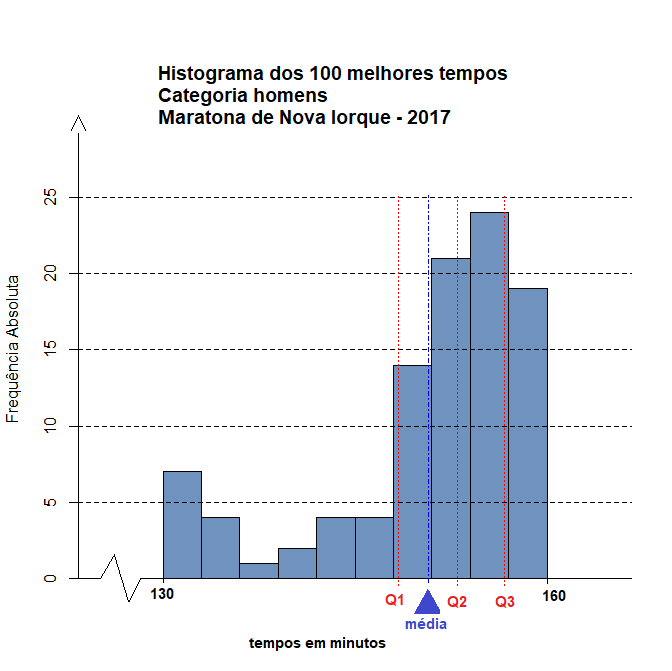
\includegraphics[width=.4\linewidth]{hist_homens_marcas.png}
\caption{Histograma dos resultados da categoria de Homens da Maratona da Cidade de Nova York do ano 2017, com média, mediana, $Q_1$ e $Q_3$ indicados}
\label{}
\end{figure}

Comparando as duas distribuições (homens e mulheres) é possível perceber que ambas têm a mesma forma com assimetria à esquerda, o que pode ser visualizado pelos histogramas. No entanto, percebe-se que a os homens são mais rápidos (todas as medidas da \hyperref[tabela-maratona-prof]{tabela \ref{tabela-maratona-prof}} são menores para os homens). Além disso, podemos notar que há mais dispersão entre as mulheres, calculando-se a amplitude amostral. Entre as mulheres, a amplitude amostral é $185{,}15-146{,}88=38{,}27$ minutos, enquanto que entre os homens é de $158{,}33-130{,}88=27,45$ minutos. Veja na \hyperref[histograma-comparando]{figura \ref{histograma-comparando}}, dois histogramas correspondentes às categorias homens e mulheres, construídos na mesma escala, ilustrando os comentários da comparação das duas categorias.

\begin{figure}[H]
\centering

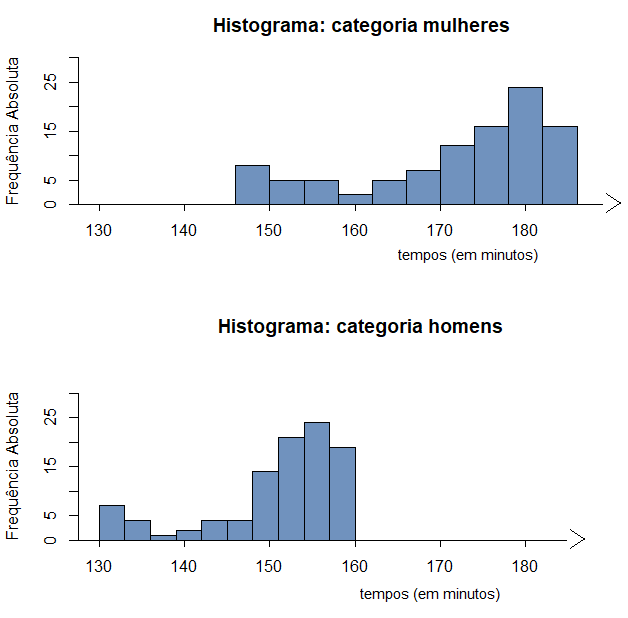
\includegraphics[width=.5\linewidth]{hist_hxm}
\caption{Histogramas dos 100 melhores tempos das categorias homens e mulheres}
\label{histograma-comparando}
\end{figure}

Observe como a comparação entre as duas categorias (homens e mulheres) é mais simples se usarmos a representação dos dados com o \hyperref[boxplot_mulheres_homens]{boxplot}.

\begin{figure}[H]
\centering

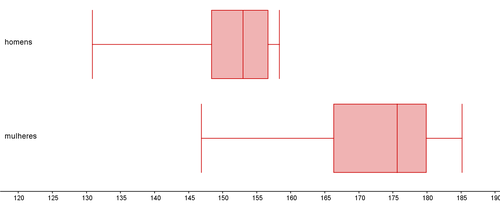
\includegraphics[width=.8\linewidth]{boxplot_mulheres_homens.png}
\caption{Boxplots dos 100 melhores tempos das categorias homens e mulheres (sem sinalização de valores discrepantes)}
\label{boxplot_mulheres_homens}
\end{figure}

\end{solucao}
\fi

\end{document}